\documentclass[a4paper,9pt]{article}
\title{Evaluation of Lulesh with SMGuard}
\date{}
\usepackage{geometry}
\usepackage{amsmath}
\usepackage{breqn}
\usepackage{pdflscape}
\usepackage{multicol}  
\usepackage{multirow} 
\usepackage{booktabs}
\usepackage{array}
\usepackage{indentfirst}
\usepackage{caption}
\usepackage{graphicx, subfig}
\setlength{\parindent}{2em}
\newcommand{\tabincell}[2]{\begin{tabular}{@{}#1@{}}#2\end{tabular}}
\geometry{a4paper,scale=0.8}

\begin{document} 
\maketitle

%\tableofcontents
Please refer to Section 6.1 of SMGuard paper for the detail information about experimental environment.

\section{Kernels in Lulesh}

\begin{table}[htbp]
	\centering
%	\footnotesize
	\small
	\caption{Kernels of Lulesh.(Problem size=100$\times$100$\times$100)}
	\begin{tabular}{p{4cm}cccccc}
		\toprule
		Kernel & Abbreviation & \multicolumn{1}{p{1cm}}{Grid size} & \multicolumn{1}{p{1cm}}{Block size} & \multicolumn{1}{p{2cm}}{Single duration(ms)} & \multicolumn{1}{p{2cm}}{Overall running time(ms)} & \multicolumn{1}{p{2cm}}{Running time ratio} \\
		\midrule
		AddNodeForcesFromElems\\\_kernel & Kernel1 & 16099 & 64    & 1.962 & 1991.092 & 6.14\% \\
		\hline
		CalcVolumeForceForElem\\s\_kernel & Kernel2 & 15625 & 64    & 14.808 & 15030.340 & 46.31\% \\
		\hline
		CalcKinematicsAndMonot\\onicQGradient\_kernel & Kernel3 & 15625 & 64    & 10.004 & 10154.035 & 31.29\% \\
		\hline
		CalcAccelerationForNod\\es\_kernel & Kernel4 & 8050  & 128   & 0.387 & 392.838 & 1.21\% \\
		\hline
		CalcPositionAndVelocit\\yForNodes\_kernel & Kernel5 & 8050  & 128   & 0.839 & 851.445 & 2.62\% \\
		\hline	
		CalcMonotonicQRegionFo\\rElems\_kernel & Kernel6 & 7813  & 128   & 1.256 & 1275.270 & 3.93\% \\
		\hline
		ApplyMaterialPropertie\\sAndUpdateVolume\_kernel & Kernel7 & 7813  & 128   & 2.309 & 2343.984 & 7.22\% \\
		\hline
		CalcTimeConstraintsFor\\Elems\_kernel & Kernel8 & 1024  & 128   & 0.402 & 408.127 & 1.26\% \\
		\hline
		ApplyAccelerationBound\\aryConditionsForNodes\_kernel & Kernel9 & 80    & 128   & 0.002 & 2.025 & 0.01\% \\
		\hline
		CalcMinDtOneBlock & Kernel10 & 2     & 1024  & 0.004 & 4.399 & 0.01\% \\
		\bottomrule
	\end{tabular}%
	\label{tab:kernels}%
\end{table}%
Table \ref{tab:kernels} shows the information of kernels in our evaluated Lulesh. There are 10 CUDA kernels used in Lulesh, and the total running time ratios of each kernel are shown in Table \ref{tab:kernels}. Kernels \emph{CalcVolumeForceForElems\_kernel} and \emph{CalcKinematicsAndMonotonicQGradient\_kernel} occupy most of overall kernel running time.

\section{Performance Improvement}

Figure \ref{fig:performance_improvement} shows the performance improvement for Lulesh over MPS with different number of reserved CapSM when corunning lulesh with different applications. When the reserved number of CapSM is 0, it means the use of GPU resource of co-location pairs is not restricted, which is actually the default MPS mechanism. When the reserved number of CapSM is 13, it means running Lulesh standalone. From the results in Figure \ref{fig:performance_improvement}, we can see that when the GPU resource is reserved, performance of Lulesh can have a great improvement in co-location scenario. And the more GPU resource is reserved for Lulesh, the better the performance. From the results we can see that SMGuard is effective for real applications like Lulesh. 

\begin{figure}[!t]
	\centering
	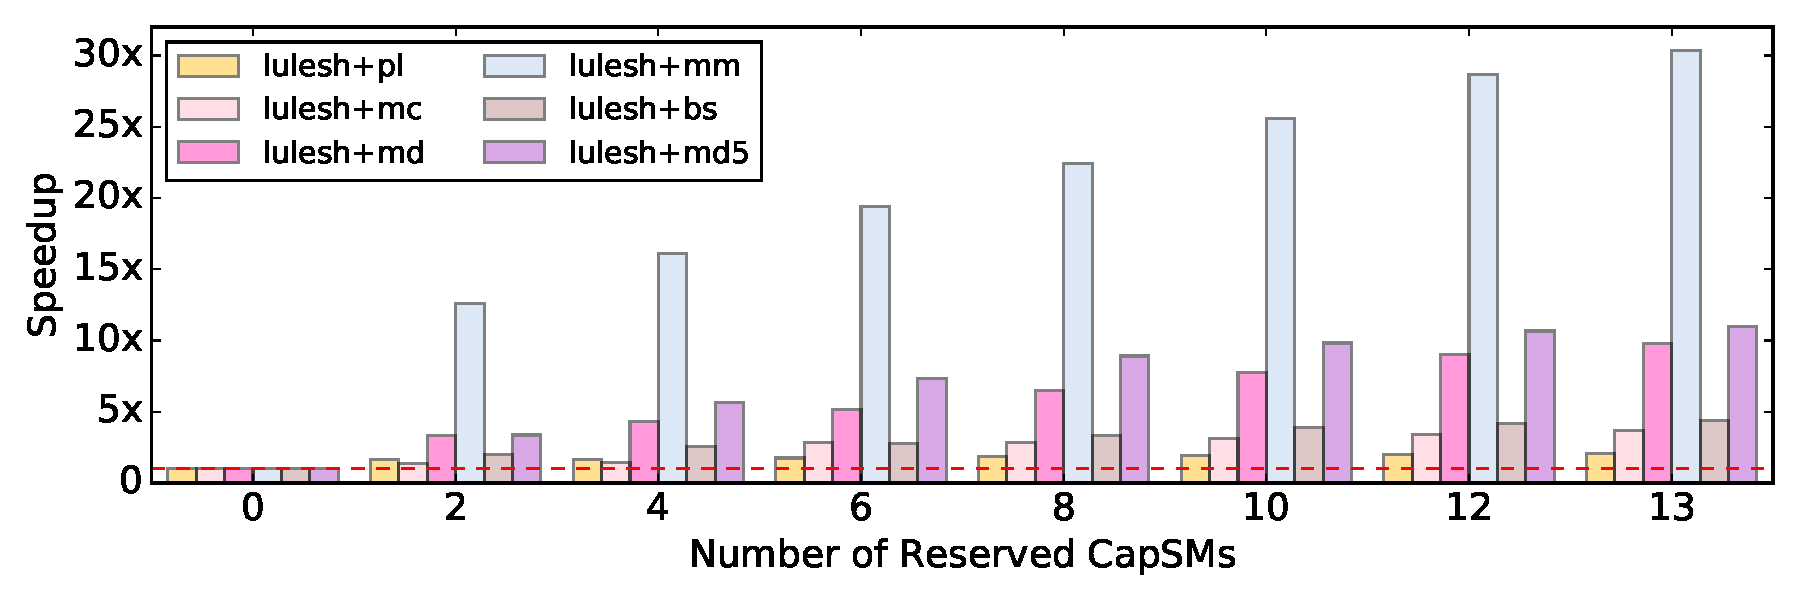
\includegraphics[width=6.5in]{fig/lulesh_performance_over_mps.pdf}
	\caption{Performance improvement for Lulesh over MPS with different number of reserved CapSM when co-running lulesh with different applications.0 reserved CapSM means the use of GPU resource of co-location pairs is not restricted; 13 reserved CapSMs means running lulesh standalone.}
	\label{fig:performance_improvement}
\end{figure}


\section{Introduced Overhead}
To evaluate the overhead introduced by SMGuard after Lulesh is transformed. we run original and transformed versions of Lulesh in standalone mode respectively. We collect the running time of each kernel in Lulesh and the overall turnaround time of all the launched kernels, then we calculate the ratio between increased running time and baseline as the introduced overhead . The results are shown in Figure \ref{fig:introduced_overhead}. We can see that the introduced overhead of most kernels of Lulesh is less than 10\%. Although the introduced overhead of kernels \emph{CalcTimeConstraintsForElems\_kernel} and \emph{ApplyAccelerationBoundaryConditionsForNodes\_kernel} is very serious, which can be as high as 395.14\%, it has negligible impact on the overall turnaround time because of the very small running time ratio of kernels \emph{CalcTimeConstraintsForElems\_kernel} and \emph{ApplyAccelerationBoundaryConditionsForNodes\_kernel} as shown in Table \ref{tab:kernels}. The introduced overhead of the overall turnaround time of Lulesh is only about 5.70\%.

\begin{figure}[!t]
	\centering
	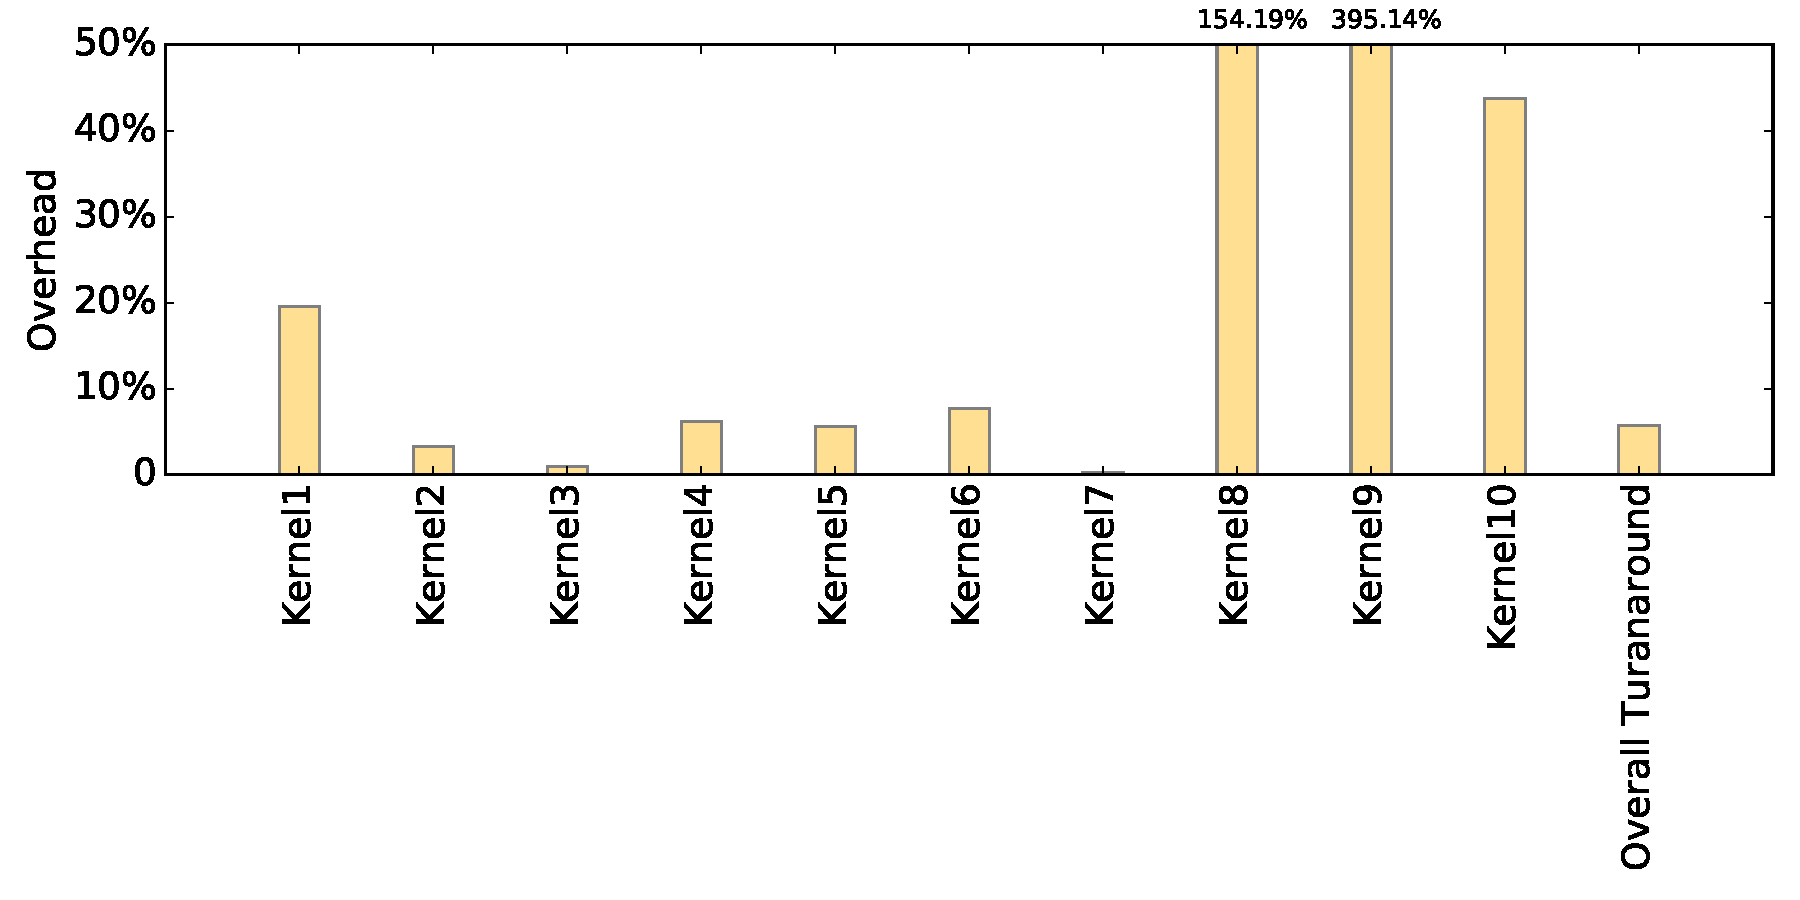
\includegraphics[width=6.5in]{fig/lulesh_introduced_overhead.pdf}
	\caption{Introduced overhead of execution time for different kernels and overall turnaround time of lulesh over baseline.}
	\label{fig:introduced_overhead}
\end{figure}
    
\end{document} 